\documentclass[a4paper, 11pt]{article}

\usepackage{amssymb}
\usepackage{amsmath}
\usepackage{graphicx}
\usepackage{setspace}
\usepackage{xcolor}
\usepackage{epstopdf}


\topmargin -10mm
\oddsidemargin 0mm
\evensidemargin 0mm
\textwidth 158mm
\textheight 226mm
\parskip 0mm

\def\Response{\noindent \textbf{Response:~}}
\newcommand{\Question}[1]{\textcolor[rgb]{0.51,0.00,0.00}{#1}}
\newcommand{\PaperText}[1]{\emph{#1}}

\title{Revision of Paper TRETS-2013-0065 Imprecise Datapath Design: An Overclocking Approach}
\author{Kan Shi, David Boland and George A. Constantinides}
\date{}

\pagenumbering{arabic}

\begin{document}
\maketitle

We thank the reviewers for their constructive comments and suggestions. We would like to offer the following response detailing the changes we have made as a result of their recommendations.

\section*{Reviewer 2}
\begin{enumerate}
  \item \Question{I believe the practical behavior is that the circuit will operate perfectly away from timing-spec corners, but that the over-clocking will simply exacerbate these. Do you believe correcting for PVT guardband by subtracting it is fair? What if arithmetic logic is more susceptible to temperature issues due to hot-spots and high toggle rate? The net effect in imprecision could be dramatically higher at process corners. I believe this should be noted/discussed (or refuted), but I think it is safe to call this future work.}
      
      \Response We would like to clarify that we run the actual (arithmetic) circuit under test on an FPGA board. So when we said in the original manuscript that we `subtract' the guard band, we meant that frequency of operation of the model is adjusted to match the observed operation. This is purely done for a fair comparison, to separate out performance boost from timing margins from error-inducing over clocking (the latter being the focus of this paper). We did not want to include the conservative timing margins within our quoted performance improvement. We have clarified this point in Section XXX in the revised manuscript.
      
  \item \Question{A second point I would make is that you seem to have an assumption that errors do not compound. What if your arithmetic is in an IIR or used in later computations? Do the principles of the paper hold when you get an imprecise data point, then multiply or divide it in some future computation?  I think that looking at a single adder in isolation is a bit optimistic.}
      
      \Response This is a good point. We have not addressed this concern theoretically to date, although we do address it empirically in the paper (see Section XXX, where several chained arithmetic units are used, including an IIR filter as suggested by the reviewer; results are in line with other benchmarks). Nevertheless, we do intend to consider the theoretical limits of this behaviour, and have added this to the future work in Section XXX. 
            
  \item \Question{A third source of inaccuracy is that most FPGA timing models include crosstalk in their guardband - i.e. don't specifically do crosstalk-aware timing analysis or glitching.  Is your modeling being optimistic by looking at a circuit in isolation?  The measured/visual empirical results would incorporate this, but the model doesn't incorporate anything like it.}
      
      \Response Again, this is a good point. We have opted for the simplest possible model to capture the notion of over clocking, and have then reverted to experimental results to verify whether the model sufficiently captures the complexity of a real implementation. For the circuits we have used, the model prediction matches well with the empirical results, as shown in Section XXX. These benchmarks are sufficiently large to have confidence that the presence of more than one basic arithmetic core does not have a significant impact on the overall behaviour (including due to crosstalk). However, it is certainly possible that the accuracy of the model degrades as the device fills up, an issue we intend to explore in future work and have added to the list of future work in Section XXX.

  \item \Question{In the introduction you claim that ``pipelining will not tend to reduce the latency of the datapath''. I don't think this is practically the case - not all paths are critical and pipelining does not imply C-slowing. For example, since a typical FPGA memory and DSP block operate grater than 500 MHz, in my preceding example you may need to pipeline some portions of the FPGA routing and logic, but you do not need to further pipeline these.}
      
      \Response Your point is valid if the pipeline stages are unequally distributed in time across the critical path, a non-ideal situation but - as you point out - a practical one, especially in FPGA implementation. An alternative way to improve latency in the case of your example would be to equally distribute the registers corresponding to the existing 10 ticks of latency, although we accept that this retiming is not always possible in FPGA designs. We have modified the comment to "assuming perfect pipeline stage balancing, further pipelining will not tend to reduce the latency of the datapath"; this can be found in Section XXX of the revised manuscript.
  
  \item \Question{Wording has some comma-itis. E.g. first sentence of the intro should not have a comma in ``demonstrated that, significant performance ...''}
      
      \Response Thanks. This has been improved, we hope.
      
  \item \Question{You don't specify the speed-grade of the Xilinx device. It might be relevant if you have a down-binned device.}
      
      \Response The precise FPGA used was a Xilinx Virtex-6 XC6VLX240T-1FFG1156 (speed grade is -1). This has now been included in Section XXX of the revised manuscript.
\end{enumerate}


\section*{Reviewer 3}
\begin{enumerate}
  \item \Question{The first sentence of the abstract is completely devoid of context, and may be the worst sentence in the entire article, given its importance. A much more appropriate sentence is the start of Section 1, Paragraph 4.}
            
      \Response We have modified the first two sentences of the abstract, which now read as follows:\\
           
      \PaperText{In this paper, we describe an alternative circuit design methodology to provide a trade-off between accuracy, performance and silicon area. We compare two different approaches that could trade accuracy for performance.}\\

  \item \Question{What are the chances that an entire design with all its complexities could be accelerated in this fashion? (i.e. Could the overall clock frequency be increased?) Imprecision may be tolerable in data, but is probably not tolerable in control.}
            
      \Response We agree. The approach is targeted at datapath logic. In our experience, the critical path of complex signal processing systems often resides in the datapath, in which case this approach would directly improve the clock frequency. In the case where the critical path lies elsewhere, it may still be possible to improve the overall operating speed of the system-level design solely by this approach, by using multiple clock domains, which may be practical in the case of large sections of datapath with simple control structures (e.g. the filters we present) that are then interfaced to more complex control at IP boundaries. We now note this in Section XXX as an area for future work.
      
  \item \Question{In Figure 1, you use $\mu$, whereas in the text and in Equation 4, you use $\mu_c$.  The converse is true for Section 7.4 and equations (35), (36), and (37).}
      
      \Response Thanks. It should be $\mu_c$ in Fig.1 and Equations (35), (36) and (37). It has been fixed.\\
      
  \item \Question{In Section 3.2, it would be helpful if you could illustrate or define your [-1,1) fixed-point format. Do you number your bits from k-1 to 0 or from 0 to k-1?}
      
      
 XXX -> Kan, THE TEXT BELOW IS NOT ANSWERING THE QUESTION! The question is simple: is your MSB labelled $a_0$ or $a_1$ or $a_k$ or $a_{k-1}$ - which order are the bits in??
      
      \Response We meant that all numbers are normalized to fractional numbers within the range [-1,1). The truncation process is illustrated in the figure below, which is not included in this manuscript due to the space limit. As seen in this figure, the original number embodies k fractional bits, while the truncated number embodies n fractional bits. Given that all bits are mutually independent and uniformly distributed, Equation (2) gives the mean value of the truncated bits. 
      
      \begin{figure}[htbp]
        \centering
        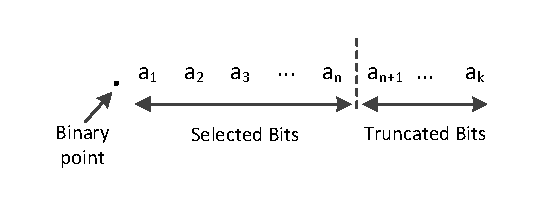
\includegraphics[width=3.2in]{./Figure/Truncation.pdf}
        %\caption{title.}
      \end{figure}
      
      We have modified the first sentence of the second paragraph of Section 3.2:\\
      
      \PaperText{If the input signal of a circuit contains $k$ fractional bits, truncation error occurs when the input signal is truncated from $k$ bits to $n$ bits.}\\
      
  \item \Question{In Section 3.3, for $A_i\neq B_i$ (Carry Propagation), you seem to be saying that $S_i = C_{i-1} = 0$.  If $A_i \neq B_i$ then $A_i + B_i = 1$, but that tells us nothing unless we know $C_{i-1}$, and it is not necessarily 0 as you claim.}
      
      \Response Thanks for pointing this out. In this case it should be $C_{i-1} =1$, because carry is propagated from bit $i-1$ to bit $i$. Hence $S_i=A_i+B_i+C_{i-1}=0$.
      
      This statement is modified as follows:\\
      
      \PaperText{Carry propagation: $A_i\neq B_i$, the carry propagates for this carry at bit $i$, and $C_{i-1}=1$, $S_i=0$.}\\
      
  \item \Question{For $A_i = B_i$ (either 0 or 1), there is no carry annihilation if their value is 1, and $S_i = C_{i-1} = 1$ seems to be a condition, not a consequence.}
      
      \Response This statement is only applied to determine the annihilation of an existing carry chain, i.e. $C_{i-1}=1$. In this case if $A_i=B_i=1$, the current carry chain is annihilated, meanwhile a new carry chain is generated. If $A_i=B_i=0$, the current carry chain is annihilated but without generating a new chain. In both situations we have $S_i=C_{i-1}=1$.

  \item \Question{In 3.2, we have $k$ as the full RCA length, and $n$ as the truncated length.  Compare that to $n$ in 3.3.2 as the length of the non-truncated but overclocked RCA.}
      
      \Response In both sections, $k$ is used to denote the word-length of the input signal, whereas $n$ is the word-length of RCA.
      
  \item \Question{Also in 3.3.2, the MSB is given as $2^n$, instead of $2^0$ as would be expected for the [-1, 1) fixed-point format you mentioned.}
      
      \Response : $2^n$ is used here because $2^i$ is used in Equation (7). Nevertheless we agree it might be confusing to put $2^n$ here, and we have changed the second paragraph of Section 3.3.2 to look as follows:\\
      
 XXX -> Kan, check this answer makes sense with reference to the one above about the format.
      
      \PaperText{For $C_{tm}$, correct results will be generated from bit $S_t$ to bit $S_{t+b-1}$. Hence the absolute value of error seen at the output, normalized to the MSB, is given by (7), where $\hat{S}_i$ and $S_i$ denote the actual value and error-free value of outputs at bit $i$, respectively.}\\
      
  \item \Question{Still in 3.3.2, you seem to be saying that when a timing error occurs, none of the bits propagate. You assume $S_{t+b}=S_{t+b+1}=\cdots=S_{t+m-2}=0$ when there is no error, and $S_{t+b}=S_{t+b+1}=\cdots=S_{t+m-2}=1$ when there is an error. I think you are assuming the worst case, where no carry propagation occurs, so it is no surprise that you comment that the magnitude of overclocking error has no dependence on the length of carry chain $m$.}
      
      \Response The value of output $S_i$ is determined based on the statements in Section 3.3.1. In this case, for carry propagation and timing error occurs, we have $S_i=A_i+B_i+C_{i-1}=A_i+B_i=1$. 
      
  \item \Question{In 3.3.4, I see the $E_O = 2^{-b}-2^{-n-1}$ result, but am puzzled by it.  At the very least, I am not sure where the $-b$ exponent is coming from, since (8) defines $e_{tm} = 2^{t+b-n}$.}
      
      \Response We would derive Equation (14) as follows:
      
      \begin{align*}
        E_O&=\sum_t\sum_m P_{tm}\cdot e_{tm}\\ &=\sum_{t=0}^{n-b}2^{t+b-n}\cdot\left(\sum_{m=b+1}^{n-t}(1/2)^{m+1}+(1/2)^{n-t+1}\right)\\
        &=\sum_{t=0}^{n-b}2^{t+b-n}\cdot\left((1/2)^{b+1}-(1/2)^{n-t+1}+(1/2)^{n-t+1}\right)\\
        &=\sum_{t=0}^{n-b}2^{t+b-n}\cdot2^{-b-1}=\sum_{t=0}^{n-b}2^{t-n-1}\\
        &=2^{-n-1}\cdot\left(2^{n-b+1}-1\right)\\
        &=2^{-b}-2^{-n-1}
      \end{align*}
      
      The detailed process is not included in the manuscript due to the space limit.
      
  \item \Question{The third and fourth paragraphs of Section 5.1 mention the 4-stage CSA, but Figure 4 does not show any data for a 4-stage CSA.}
      
      \Response Thanks. In the third paragraph of Section 3.1, it should be the 3-stage CSA. The last sentence of this paragraph has been revised as:\\
      
      \PaperText{Although the CSA with 3 stages is best for some frequencies, the overclocked RCA is still the optimum design when high operating frequencies are applied.}\\
      
      The 4-stage CSA is introduced in the fourth paragraph and Fig. 5 and Fig. 6, where we consider a variety of area constraints. Ideally with larger available area, CSA with more stages will be included in both Fig. 5 and Fig. 6. However the general trend will be similar. In previous paragraphs of this section, we only use 2-stage CSA and 3-stage CSA as examples to illustrate the design method. We have clarified this point by adding the following sentence to the fourth paragraph of Section 5.1:\\
      
      \PaperText{We implement CSA with all possible stage numbers within the given area specification.}\\
      
  \item \Question{In the experimental setup, I would be curious to know whether you used any particular constraints on the circuits-under-test to enhance their chances of success.}
      
      \Response  No specific constraints are applied, except the global clock constraint.
      
  \item \Question{May I assume that your figures will be colorized?}
        
      \Response Yes, Fig.~3, Fig.~4 and Fig.~10 will be colorized in the final manuscript.
      
  \item \Question{An incomplete list of spelling or grammar or punctuation comments.}
      
      \Response Thanks, they have been revised.

      

\end{enumerate}




\end{document}